\begin{frame}
    \frametitle{Visualizzare ed Elaborare documenti XML}
    \addtocounter{nframe}{1}
    
    %\begin{center}
    %    
\includegraphics[width=.2\textwidth]{../imgs/tei-r.pdf}
    %\end{center}
    %\textit{In parte già disponibili nei moduli TEI di base}

     \begin{block}{Documenti Object Model (DOM)}
        The Document Object Model (DOM) is an application programming interface (API) for XML.
        \\ The DOM maps out an entire XML document as a hierarchy of nodes.

    %     \emph{Per la critica testuale indispensabili i moduli}
        %  \begin{itemize}
        %     \item Controllare la codifica e correggere i refusi
        %     \item Assicurarsi che tutto sia stato trascritto correttamente
        %     \item Mostrare il testo a persone che non conoscono XML-TEI
        %     \item Disporre di una versione del lavoro fruibile
        % \end{itemize}
     \end{block}


    
\end{frame}


\begin{frame}
    \frametitle{Visualizzare ed Elaborare documenti XML}
    \addtocounter{nframe}{1}
    
    \begin{center}
        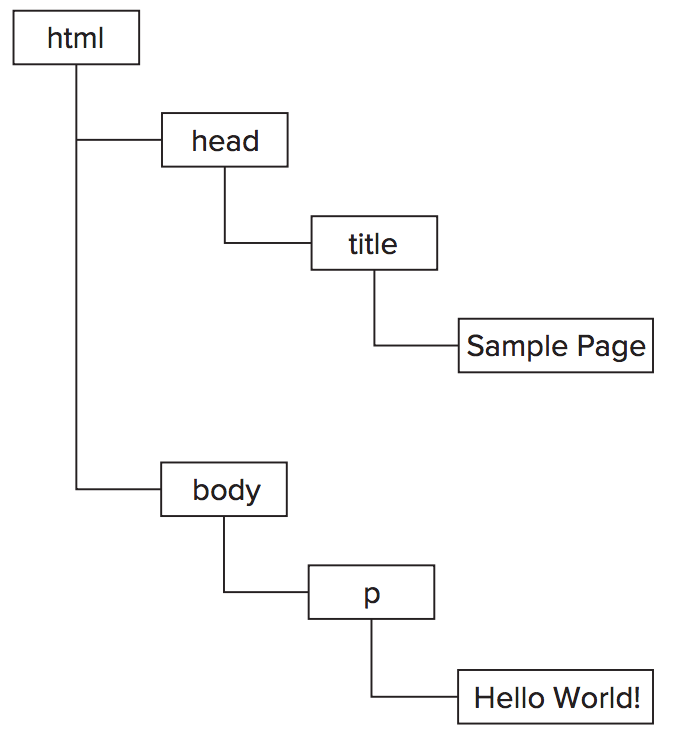
\includegraphics[width=.9\textwidth]{imgs/XML-DOM.png}
    \end{center}
    \textit{In parte già disponibili nei moduli TEI di base}

\end{frame}

% The Document Object Model
% The document object model (DOM) is, as previously mentioned, a way of representing the document
% independent of browser type. It allows a developer to access the document via a common set of objects,
% properties, methods, and events, and to alter the contents of the web page dynamically using scripts.
% You should be aware that some small variations are usually added to the DOM by the browser
% vendor. So, to guarantee that you don’t fall afoul of a particular implementation, the W3C has
% provided a generic set of objects, properties, and methods that should be available in all browsers, in
% the form of the DOM standard.
% The DOM Standard
% We haven’t talked about the DOM standard so far, and for a particular reason: It’s not the easiest
% standard to follow. Supporting a generic set of properties and methods has proved to be a very
% complex task, and the DOM standard has been broken down into separate levels and sections
% to deal with the different areas. The different levels of the standard are all at differing stages of
% completion.

% Level 0
% Level 0 is a bit of a misnomer, because there wasn’t really a level 0 of the standard. This term in fact
% refers to the “old way” of doing things—the methods implemented by the browser vendors before the
% DOM standard. Someone mentioning level 0 properties is referring to a more linear notation of accessing
% properties and methods. For example, typically you’d reference items on a form with the following code:
% document.forms[0].elements[1].value = "button1";
% We’re not going to cover such properties and methods in this chapter, because they have been
% superseded by newer methods.

% Level 1
% Level 1 is the first version of the standard. It is split into two sections: One is defined as core
% (objects, properties, and methods that can apply to both XML and HTML) and the other as HTMLThe Document Object Model
% ❘ 235
% (HTML‐specific objects, properties, and methods). The first section deals with how to go about
% navigating and manipulating the structure of the document. The objects, properties, and methods in
% this section are very abstract. The second section deals with HTML only and offers a set of objects
% corresponding to all the HTML elements. This chapter mainly deals with the second section—
% level 1 of the standard.
% In 2000, level 1 was revamped and corrected, though it only made it to a working draft and not to a
% full W3C recommendation.

% Level 2
% Level 2 is complete and many of the properties, methods, and events have been implemented
% by today’s browsers. It has sections that add specifications for events and style sheets to the
% specifications for core and HTML‐specific properties and events. (It also provides sections on
% views and traversal ranges, neither of which is covered in this book; you can find more information
% at www.w3.org/TR/2000/PR‐DOM‐Level‐2‐Views‐20000927/ and www.w3.org/TR/2000/
% PR‐DOM‐Level‐2‐Traversal‐Range‐20000927/ .)

% Level 3
% Level 3 achieved recommendation status in 2004. It is intended to resolve a lot of the complications
% that still exist in the event model in level 2 of the standard, and adds support for XML features,
% such as content models and being able to save the DOM as an XML document.
% Level 4
% In May 2014, DOM level 4 reached candidate recommendation status. It consolidates DOM level 3
% with several independent components. At the time of this writing, no modern browser supports
% DOM level 4, although that will change in the future.